\documentclass[12pt,a4paper]{article}
\usepackage[utf8]{inputenc}
\usepackage{graphicx}
% Document config
\usepackage[letterpaper, margin=1in]{geometry}
\usepackage[spanish]{babel}
\usepackage[utf8]{inputenc}
\usepackage{tikz}
\usepackage{hyperref}
\usepackage{minted,xcolor}
\usemintedstyle{tango}
\usepackage{color}
\usepackage{xcolor}
\usepackage{float}
\usepackage{tcolorbox}
\usepackage[nottoc]{tocbibind}
\usepackage{graphicx}
\usepackage{listings}
\usepackage{lineno}
\usepackage{fancyvrb}
\usepackage{minted}
\usepackage[utf8]{inputenc}
\usepackage{pdfpages} %para importar paginas de un pdf
\usepackage{multirow}
\addto\captionsspanish{\renewcommand{\listtablename}{Índice de tablas}}		% Cambiar nombre a lista de tablas   
\addto\captionsspanish{\renewcommand{\tablename}{Tabla}}					% Cambiar nombre a tablas
\usepackage{float}		% Para ubicar las tablas y figuras justo después del texto
\usepackage{pdfpages}
\usepackage{enumerate}%listas y viñetas

\usepackage{parskip}
\usepackage{circuitikz}
\usepackage{siunitx}
\usepackage{hyperref}
%%%%%%%%%%%%%%%%%%%%%%%%%%%%%%%%%%%%%%%%%%%%%%%%%%%%%%%%%%%%%%%%%%%%
\title{
{

    \begin{tikzpicture}[overlay, remember picture]
        \node[anchor=north west, %anchor is upper left corner of the graphic
            xshift=3cm, %shifting around
            yshift=-4cm] 
            at (current page.north west) %left upper corner of the page
        {
\includegraphics[height=1.3cm]{logoEIE.png}}; 
    \end{tikzpicture}
    \begin{tikzpicture}[overlay, remember picture]
        \node[anchor=north east, %anchor is upper left corner of the graphic
            xshift=-2.5cm, %shifting around
            yshift=-4cm] 
            at (current page.north east) %left upper corner of the page
        {
\includegraphics[height=1.3cm]{logoUCR.png}}; 
    \end{tikzpicture}
    \Large 
        \textbf{Universidad de Costa Rica}\\
        Facultad de Ingeniería\\
        Escuela de Ingeniería Eléctrica\\~\\ \vspace{2cm}
        \texttt{IE-0117}\\Programación Bajo Plataformas Abiertas \\
    }
    ~\\~\\
    {\LARGE \textbf{Laboratorio \#6 \vspace{0cm}}}}
    
\author{Fernando Jiménez Ureña B74020\\}
\\
\date{II ciclo\\Noviembre 2021 } 

%%%%%%%%%%%%%%%%%%%%%%%%%%%%%%%%%%%%%%%%%%%%%%
\usepackage{fancyhdr}
\pagestyle{fancy}
\setlength{\headheight}{14.49998pt}

\lhead{IE0117-Programación Bajo Plataformas Abiertas}
\chead{}
\rhead{Laboratorio \#6}
\lfoot{Universidad de Costa Rica}
\cfoot{\thepage}
\rfoot{Escuela de Ingeniería Eléctrica}
%%%%%%%%%%%%%%%%%%%%%%%


%%%%%%%%%%%%%%%%%%%%%%%%%%%%%%%%%%%%%

\begin{document}
%%%%%%%%%%%%%%%%%%%%%%%%%%%%%%%%%%%%%%%%%%%%%%%%%%%%%%%%%%%
\maketitle
\thispagestyle{empty}%%no formato a la portada
\renewcommand{\thepage}{\roman{page}}
\newpage
%%%%%%%%%%%%%%%%%%%%%%%%%%%%%%%%%%%%%%%%5
\renewcommand{\thepage}{\arabic{page}} 
\setcounter{page}{1}

\newpage


%%%%%%%%%%%%%%%%%%%%%%%%%%%%%%%
\newpage
\section{Resumen}

En el presente laboratorio se estudian de manera teórica y práctica importantes conceptos que son esenciales para la programación como lo son los Compiladores, Depuración y la Automatización de proyectos. Además se dedica una sección a los punteros en C que conforman una parte indispensable en el aprendizaje y desarrollo en dicho lenguaje.

\section{Nota Teórica}

Es importante conocer varios conceptos para el mejor entendimiento y desarrollo de este laboratorio. Uno de los conceptos que más se desarrollará a lo largo del laboratorio son los compiladores. Un compilador es un Software que traduce un programa escrito en un lenguaje de programación de alto nivel (C / C ++, COBOL, etc.) en lenguaje de máquina. [1]

El comando \textit{make} en Linux es una gran herramienta para facilitar la compilación de los programas que se van creando. Es un comando muy inteligente ya que logra reconocer qué archivos deben recompilarse, guarda los comandos de compilación con todos sus parámetros para encontrar librerías, ficheros de cabecera (.h), entre otros. Este comando se vuelve de gran utilidad cuando existen gran cantidad de ficheros fuente repartidos entre diferentes directorios. [2]

Luego, otro concepto importante es la depuración de programas con \textit{gdb}. El proceso de depuración es aquel que se sigue para quitar errores en el código. Un depurador, como es el caso de \textit{gdb}, es una herramienta de desarrollo muy especializada que se asocia a la aplicación en ejecución y permite inspeccionar el código. [3]

Finalmente, para este laboratorio se implementará el uso de punteros. Un puntero es una variable que contiene una dirección de memoria los cuales se definen mediante como por ejemplo \textit{tipo * nombre} : donde nombre es el identificador de la variable puntero, y tipo se refiere al tipo de variable a la que apunta [4].




\section{Análisis de Resultados}

\subsection{Compiladores}

\begin{enumerate}
    \item En su forma más general, en una sola palabra, ¿qué es un compilador?

    Traductor
    
    \vspace{35mm}
    
    \item Por medio de un diagrama, represente la principal diferencia entre un interprete y un compilador.
    
    En la Figura 1. se observa el diagrama mostrando las principales diferencias entre un intérprete y un compilador. La información contenida en dicho diagrama fue obtenida de [5].
    
    \begin{figure}[H]
    \centering
    \center
    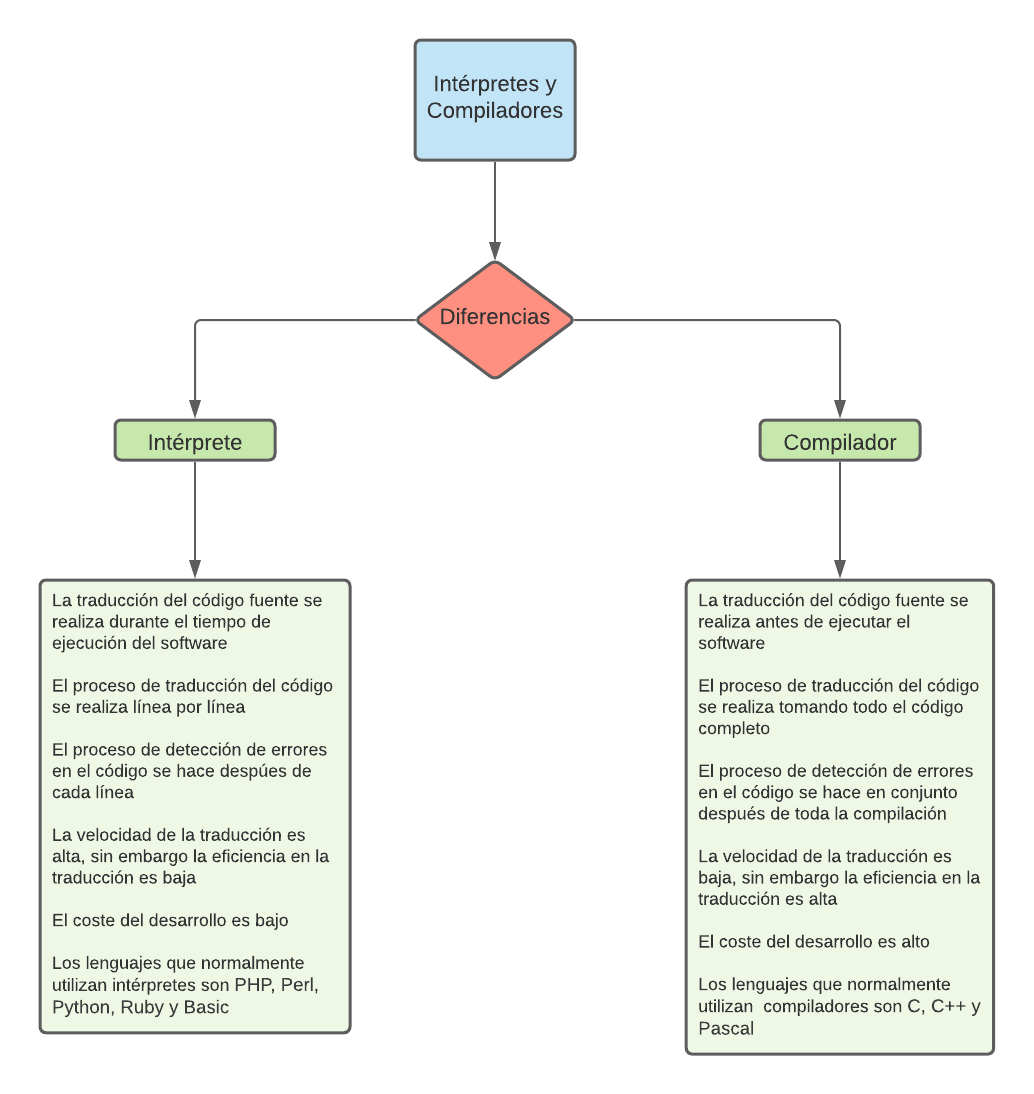
\includegraphics[width=0.9\textwidth]{Fotos_Lab6/Interpretes y compiladores.png}
    \caption{Diagrama sobre las diferencias entre un intérprete y un compilador}
    \label{1}
\end{figure}
    
    \vspace{60mm}
    
    \item Explique brevemente con una o más razones por qué un lenguaje compilado puede ser más eficiente que uno interpretado.
    
    Se puede decir que es más eficiente el uso de un compilador por encima de un intérprete ya que una vez que se compila el código fuente, el compilador proporciona al procesador, el código máquina completo y ya listo para ser ejecutado. Esto hace que sea un proceso más robusto y una vez finalizada la compilación, se tenga toda la información a mano de cualquier error encontrado en el programa. A diferencia de un intérprete que hace el proceso de la traducción del código línea por línea, por lo que se detiene cada vez que encuentre un error en una línea y así sucesivamente por lo que puede volverse tedioso encontrar todos los errores finales en el programa, por lo que se puede decir que mediante un intérprete el proceso de traducción es poco eficiente y la velocidad en la ejecución es lenta [5]
    
    \item ¿A qué se le conoce como cross-compiler?
    
    Un cross-compiler o compilador cruzado como se le conoce en español, es una herramienta bastante útil y poderosa en el desarrollo de software. Es un programa que es capaz de producir código ejecutable que se puede ejecutar en una plataforma que actualmente no es la plataforma residente para el compilador. Esto es bastante útil cuando el desarrollador necesita distribuir su programa en distintas plataformas ya que le permite mejorar el manejo de las funciones informáticas y le ayuda a superar barreras como cuando ciertos computadores en un sistema integrado posee una cantidad limitada de recursos ya que logra crear una ejecución interrelacionada entre varios componentes del sistema. [6]
    
    \item Enumere los 5 elementos que componen la estructura típica de un compilador.
    
    \begin{enumerate}
    
    \item Análisis Léxico 
    
    \item Parser / Análisis sintáctico 
    
    \item Análisis semántico 
    
    \item Optimizaciones
    
    \item Generación de código
    
    \end{enumerate}

\item Describa brevemente la función que realiza, en el proceso de compilación, cada uno de los elementos mencionados en el punto anterior.

\begin{enumerate}
    
    \item Análisis Léxico: Reconoce las palabras provenientes del código fuente y las separa en tokens.
    
    \item Parser / Análisis sintáctico: En esta sección de la compilación, el compilador entiende la estructura de las oraciones por lo que logra reconocer la función de cada palabra. Finalmente se procede a agrupar las palabras en estructuras de alto nivel.
    
    \item Análisis semántico: Es el proceso más complicado para el compilador ya que necesita interpretar de alguna manera lo que un usuario quiere decir en el código fuente. Esta parte del proceso lleva un análisis semántico bastante limitado e intenta encontrar inconsistencias.
    
    \item Optimizaciones: Este proceso es el que intenta hacer el programa lo más 'económico' posible, ya que hace que el programa corra más rápido y al mismo tiempo hace que utilice menos memoria, menos potencia requerida, menos accesos a base datos y limita el uso de la red
    
    \item Generación de código: Esta es la parte final en el proceso de compilación ya que aquí es donde se genera el código objeto 
    
    \end{enumerate}
    
\end{enumerate}

\subsection{Depuración: gdb}

\begin{enumerate}

\item ¿Cuál es la bandera del compilador gcc que se utiliza para generar un código que tenga los componentes
necesarios para depurar (debugging)?

La bandera que se utiliza para generar un código que tenga los componentes necesarios para depurar en el compilador gcc es \textit{-g}. Un depurador, en este caso \textit{-g} se utiliza para detectar errores de ejecución en un programa en C que ha compilado sin problemas. Este depurador ejecuta el programa línea a línea mostrando al mismo tiempo el código fuente y el valor de las variables. [7]

\item ¿Cuál es la línea de comandos en terminal necesaria para compilar con gcc un código fuente con el nombre fuente.c en un ejecutable llamado bin capaz de ser depurado con gdb?

gcc -g -o bin fuente.c

\item Describa brevemente para que sirven los siguientes comandos en gdb:
    \begin{enumerate}
    
    \item run: Este comando inicia el programa corrido bajo gdb. Cabe destacar que el programa que se inicia es el que se ha seleccionado previamente con el comando de archivo, o en la línea de comando de Unix cuando se inició gdb. [8]
    
    \item break: El comando break se utiliza como un punto de detenimiento donde se desea que el programa se detenga temporalmente en la ejecución para poder verificar en que momento el programa está teniendo errores o para chequear los valores de las variables. [8]
    
    \item quit: Este comando es utilizado para salir de GDB
    
    \item continue: Este comando se utiliza para que el programa siga corriendo luego de haberlo detenido en un punto de detenimiento. [8]
    
    \item print: Este comando se encarga de imprimir el valor de la expresión que puede ser por ejemplo el nombre de una variable. Se pueden agregar argumentos luego del comando para imprimir únicamente un intervalo especifico de líneas por ejemplo las primeras 25 líneas del programa. [8]
        
    \end{enumerate}


\end{enumerate}

Luego, se procede a a realizar la depuración del programa \textit{serie.c} brindado en el enunciado del laboratorio. Primero como se puede apreciar en la Figura 2., se intentó compilar de manera normal el programa con gcc y su argumento \textit{-g} y se puede observar que se detectaron múltiples errores en el programa.

\begin{figure}[H]
    \centering
    \center
    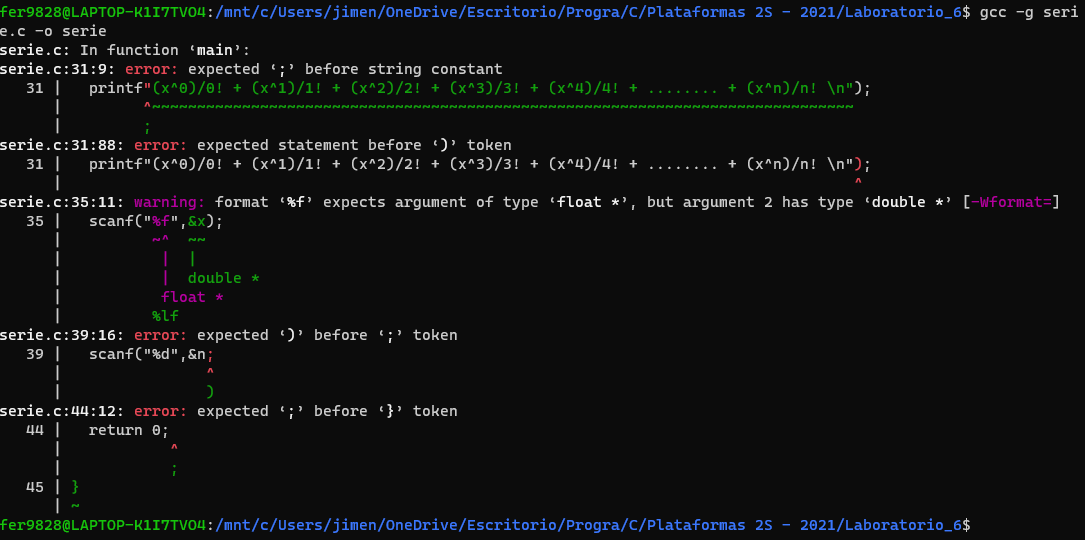
\includegraphics[width=0.9\textwidth]{Fotos_Lab6/Figura2.png}
    \caption{Compilación y errores hallados con el compilador gcc}
    \label{1}
\end{figure}

Se deben realizar las correcciones mostradas en la terminal para que se pueda generar el archivo ejecutable. Este archivo ejecutable es vital debido a que para utilizar el depurador gbd, éste únicamente detecta archivos ejecutables para poder realizar el proceso de depuración. 

Luego de realizar las debidas correcciones, se puede apreciar en la Figura 3. que se logró crear correctamente el archivo ejecutable.

\begin{figure}[H]
    \centering
    \center
    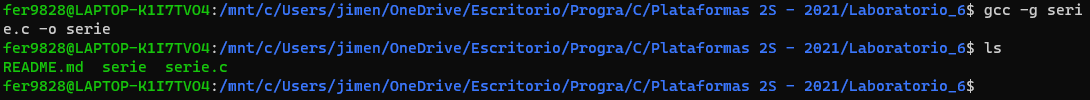
\includegraphics[width=0.9\textwidth]{Fotos_Lab6/Figura3.png}
    \caption{Ejecutable \textit{serie} creado correctamente}
    \label{1}
\end{figure}

Se procede a ejecutar el programa, y se puede observar en la Figura 4. que efectivamente si se logra correr. Sin embargo una vez que se introducen los valores solicitados por el programa, la serie siempre dará como resultado \textit{inf}. Por lo que en este caso, es ideal depurar el programa para encontrar qué está fallando a pesar de que el programa pueda ser ejecutado en la terminal. 

\begin{figure}[H]
    \centering
    \center
    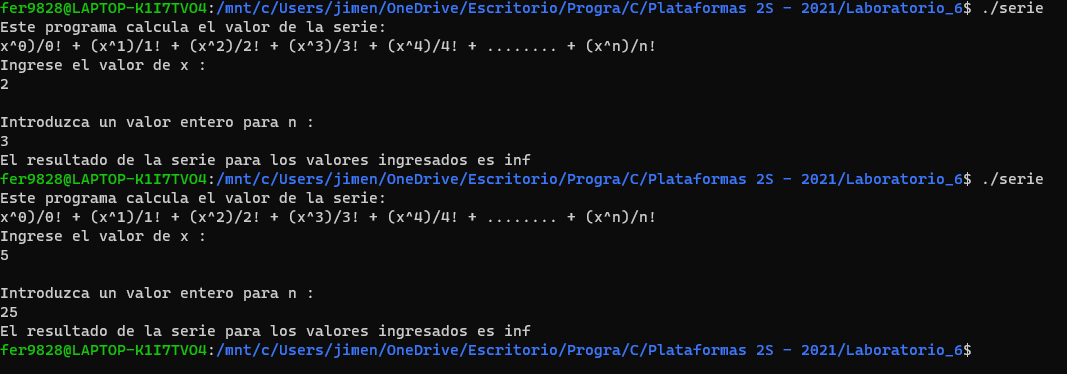
\includegraphics[width=0.9\textwidth]{Fotos_Lab6/Figura4.png}
    \caption{Ejecutable \textit{serie} creado correctamente}
    \label{1}
\end{figure}

Se procede a ejecutar el depurador GBD para analizar más a fondo cuál es la raíz de este problema. En la Figura 5. se selecciona un \textit{breakpoint} en la línea 41 donde se encuentra la expresión 'double valorserie = CalcularValorSerie(x, n);' 

\begin{figure}[H]
    \centering
    \center
    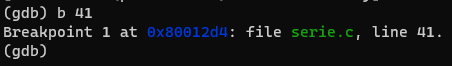
\includegraphics[width=0.9\textwidth]{Fotos_Lab6/Figura5.png}
    \caption{Eligiendo el breakpoint}
    \label{1}
\end{figure}

Luego, se procede a utilizar el comando \textit{run} y se puede observar como el depurador ejecuta el programa y pide los valores al usuario. En este caso se utilizarán los valores de x = 2 y n = 3 que se espera que devuelva el valor de 5. Una vez ejecutado como se aprecia en la Figura 6., que el programa se detiene en el breakpoint que se eligió anteriormente.

\begin{figure}[H]
    \centering
    \center
    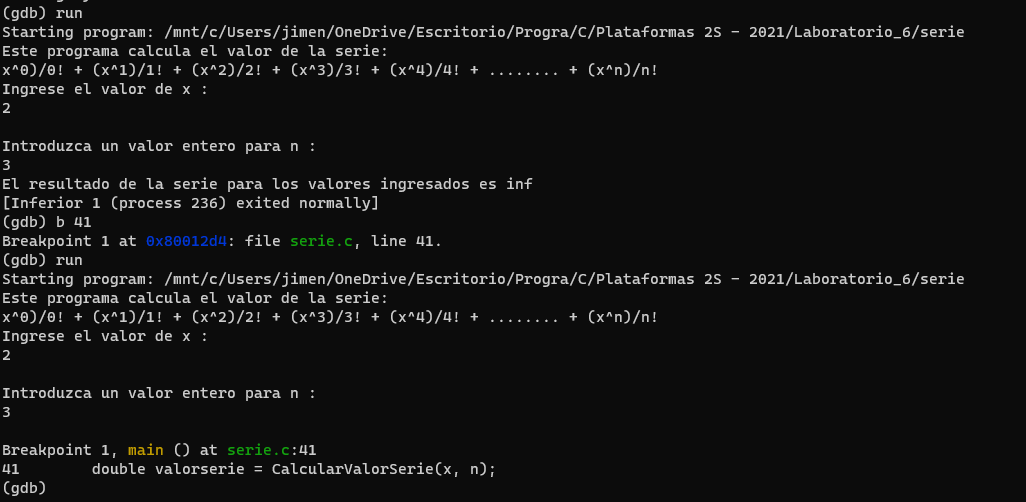
\includegraphics[width=0.9\textwidth]{Fotos_Lab6/Figura6.png}
    \caption{Ejecutando el depurador gdb}
    \label{1}
\end{figure}

Se procede a entrar a la función CalcularValorSerie() mediante el comando \textit{step} y utilizando también el comando \textit{next} hasta llegar a la función CalcularFactorial(). En la Figura 7. se observa la manera ne que se llegó a esta última función y además se puede observar mediante el comando \textit{backtrace} o \textit{bt} en cual lugar nos encontramos en ese momento.

\begin{figure}[H]
    \centering
    \center
    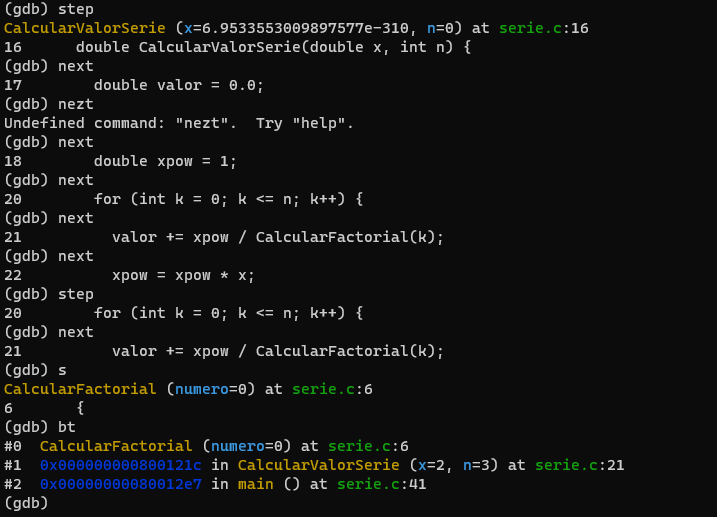
\includegraphics[width=0.9\textwidth]{Fotos_Lab6/Figura7.png}
    \caption{Entrando a la función y uso del comando backtrace}
    \label{1}
\end{figure}

Finalmente se sigue recorriendo el programa con el comando \textit{next} o abreviado \textit{n} y se llega hasta al valor de la variable 'fact' donde utilizando el comando \textit{print} se puede concluir que el valor de dicha variable nunca cambia y esto es lo que está generando el problema. Esto puede observarse en la Figura 8.

Observando más a fondo, en la operación 'fact = fact * j', 'fact' a la hora de ser inicializada en 0 esta operación nunca podrá avanzar y se concebirá el error. Por lo que 'fact' debe ser inicializada en 1 para que el ciclo for pueda utilizar los valores correctos a la hora de ser ejecutado.

\begin{figure}[H]
    \centering
    \center
    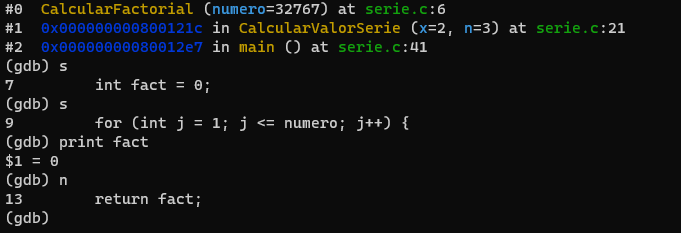
\includegraphics[width=0.9\textwidth]{Fotos_Lab6/Figura8.png}
    \caption{Analizando la variable \textit{fact}}
    \label{1}
\end{figure}

Ya una vez encontrado el error, se procede a corregirlo y en la línea 7 del código fuente se procede a cambiar el valor de 'fact' a igual a 1. Se procede a compilar nuevamente el programa y a realizar la misma prueba con los valores de x = 2 y n = 3.

\begin{figure}[H]
    \centering
    \center
    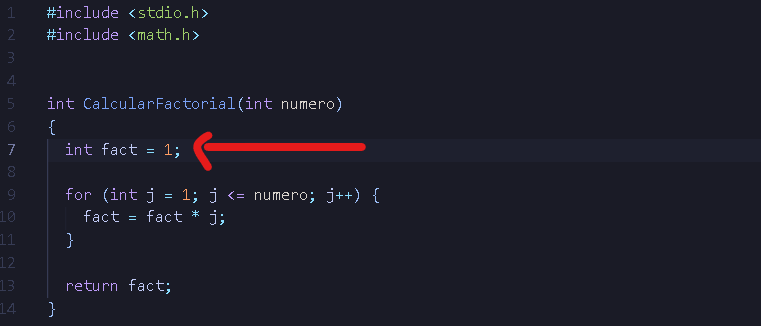
\includegraphics[width=0.9\textwidth]{Fotos_Lab6/Figura9.png}
    \caption{Arreglando el valor de la variable \textit{fact}}
    \label{1}
\end{figure}

\begin{figure}[H]
    \centering
    \center
    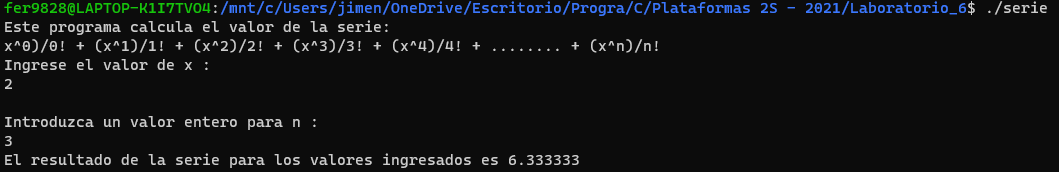
\includegraphics[width=0.9\textwidth]{Fotos_Lab6/Figura10.png}
    \caption{Compilación y ejecución del programa}
    \label{1}
\end{figure}

Como se puede observar en la Figura 9. y Figura 10. luego de realizar el cambio, finalmente el programa logra retornar el valor deseado y se arregló el problema.

\subsection{Punteros}

\subsubsection{Punteros Simples}

Para este problema, se desarrolló todo en un mismo programa sin embargo dividiéndolo en 3 funciones diferentes: La función \textit{CambioPorValor} donde se implementó un algoritmo acudiendo a una variable auxiliar encargada de hacer el cambio del valor de las variables, luego la función \textit{CambioPorPuntero} realiza un proceso similiar sin embargo acudiendo al uso de punteros y finalmente la función \textit{main} se encarga de llamar a las dos funciones y de pasarles los parámetros e imprimir el resultado del intercambio.

Se puede observar en las siguientes Figuras el código implementado y que efectivamente si se logró resolver el problema planteado.

\begin{figure}[H]
    \centering
    \center
    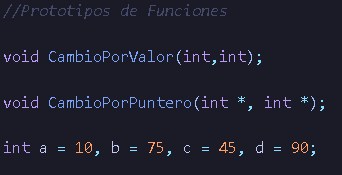
\includegraphics[width=0.9\textwidth]{Fotos_Lab6/Prototipo.png}
    \caption{Prototipo de las funciones y declaración de variables globales}
    \label{1}
\end{figure}

\begin{figure}[H]
    \centering
    \center
    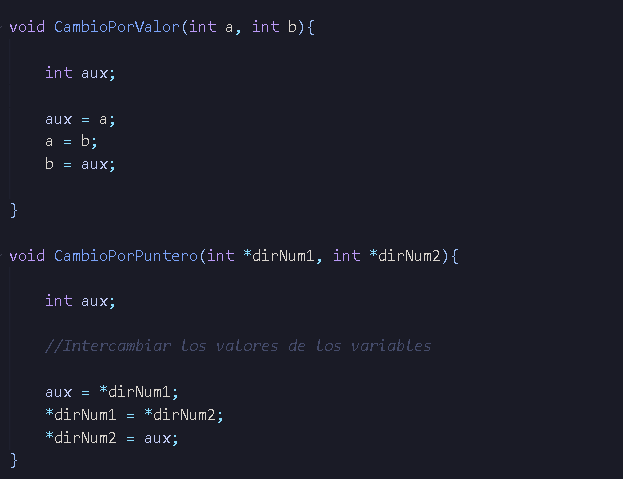
\includegraphics[width=0.9\textwidth]{Fotos_Lab6/Funciones.png}
    \caption{Funciones para desarrollar el problema}
    \label{1}
\end{figure}

\begin{figure}[H]
    \centering
    \center
    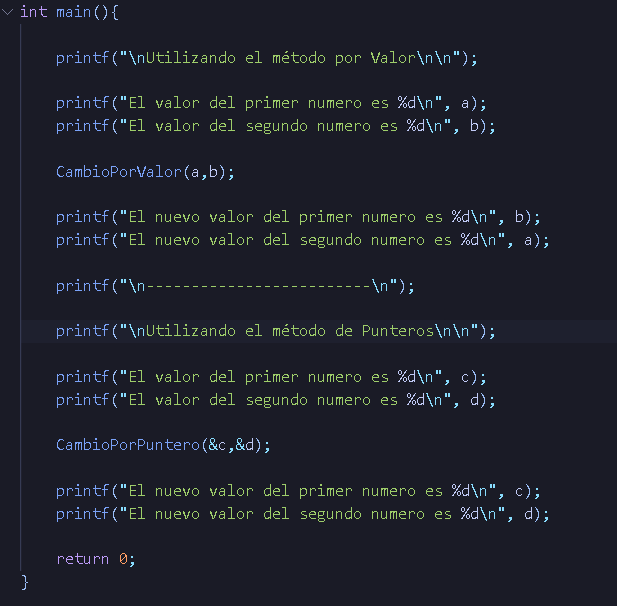
\includegraphics[width=0.9\textwidth]{Fotos_Lab6/Funcion_main.png}
    \caption{Función \textit{main}}
    \label{1}
\end{figure}

\begin{figure}[H]
    \centering
    \center
    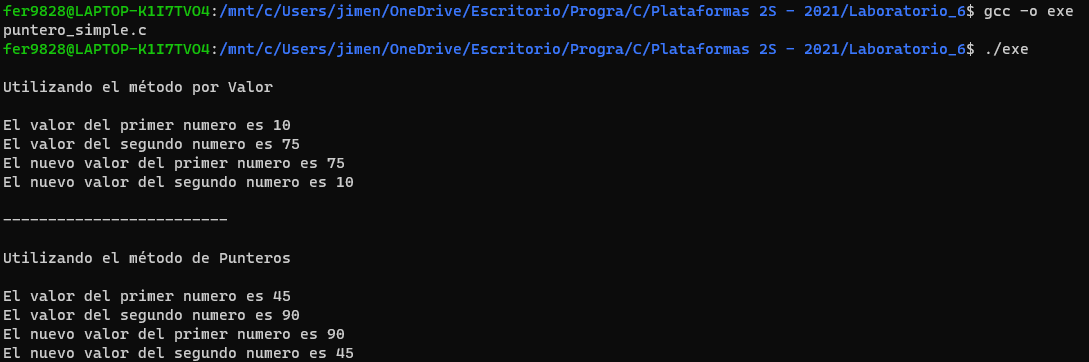
\includegraphics[width=0.9\textwidth]{Fotos_Lab6/Resultado1.png}
    \caption{Resultados Obtenidos}
    \label{1}
\end{figure}

\subsubsection{Punteros, funciones y matrices}

Para este problema, se implementaron dos funciones: \textit{armarMatriz} y \textit{mostrarMatriz}. En estas funciones se genera la matriz 10x10 con los numeros aleatorios y luego se imprime en pantalla como se aprecia en la Figura 15. y Figura 16. respectivamente

\begin{figure}[H]
    \centering
    \center
    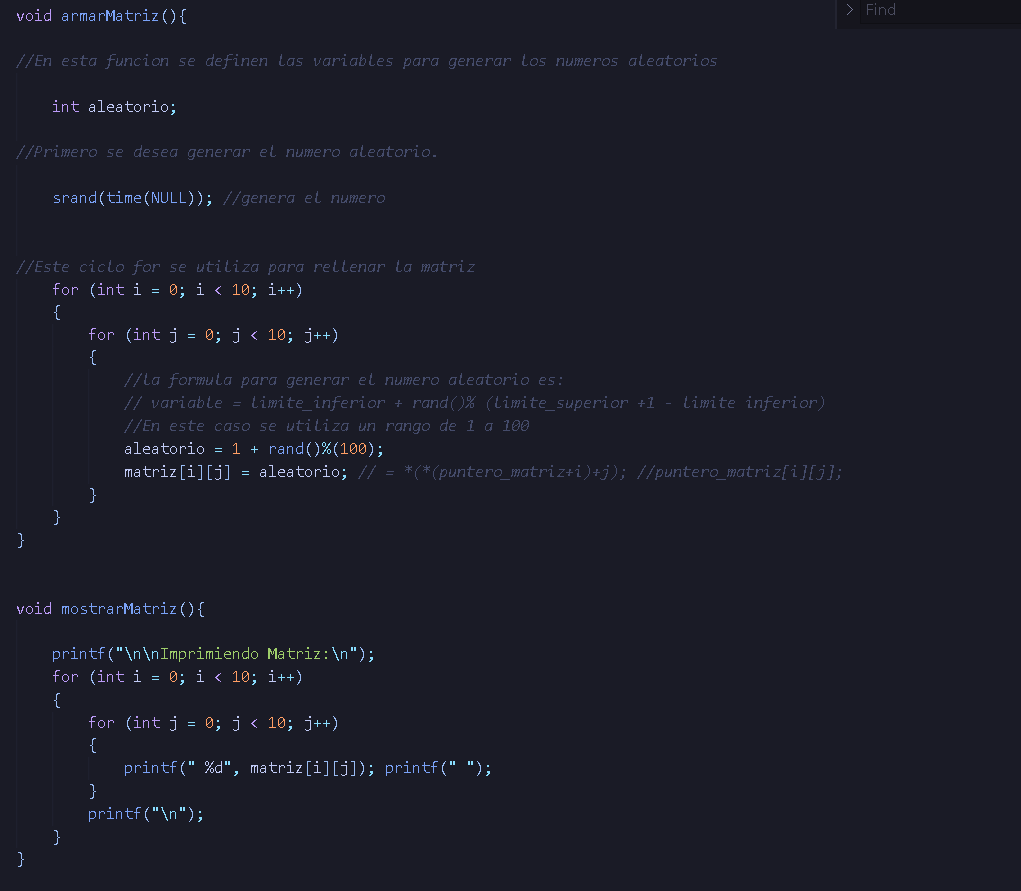
\includegraphics[width=0.9\textwidth]{Fotos_Lab6/Figura15.png}
    \caption{Funciones para generar la matriz de números aleatorios}
    \label{1}
\end{figure}

\begin{figure}[H]
    \centering
    \center
    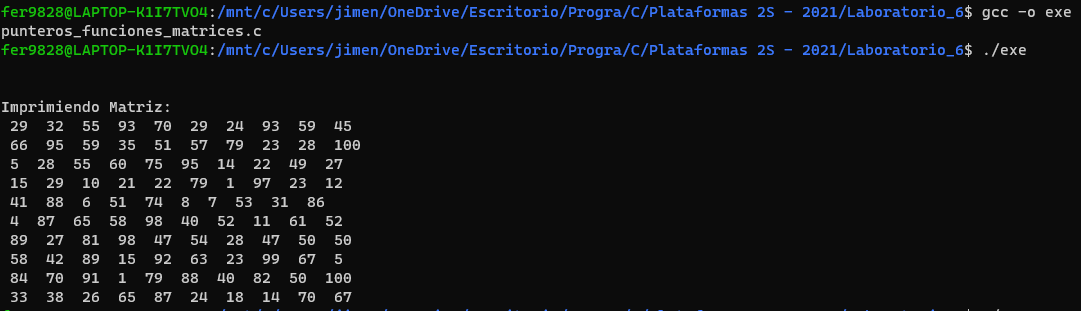
\includegraphics[width=0.9\textwidth]{Fotos_Lab6/Figura16.png}
    \caption{Matriz Impresa}
    \label{1}
\end{figure}

Es importante notar que no se logró resolver en su totalidad el problema ya que no se pudo encontrar la manera de definir la función \textit{buscar}. Por lo que únicamente se obtuvo las funciones para generar la raíz de números aleatorios e imprimirla.

\section{Conclusiones y Recomendaciones}

Para concluir es importante reconocer la importancia de haber puesto en práctica conceptos como la depuración de un programa, la automatización de proyectos con el uso del comando \textit{make}, así como reconocer las diferencias entre un compilador y un intérprete. Esto logra desarrollar buenos hábitos de programación así como la facilitación del mismo y ahorrar tiempo y recursos. Además, se lograron desarrollar diversos ejercicios con Punteros que fueron de gran utilidad para el entendimiento de este tema. 

\section{Referencias}

[1] Calvo, J. (2021). ¿Que es un Compilador en programación? – Blog Europeanvalley. Europeanvalley.es. Retrieved 16 November 2021, from https://www.europeanvalley.es/noticias/que-es-un-compilador-en-programacion/.

[2] Conceptos básicos de make y los Makefile. Chuidiang.org. (2021). Retrieved 17 November 2021, from http://www.chuidiang.org/clinux/herramientas/makefile.php#resumen.

[3] ¿Qué es la depuración? - Visual Studio (Windows). Docs.microsoft.com. (2021). Retrieved 17 November 2021, from https://docs.microsoft.com/es-es/visualstudio/debugger/what-is-debugging?view=vs-2022.

[4] A.Serrano."Introduccion al lenguaje C". Recuperado de https://blog.utp.edu.co/
jnsanchez/files/2011/03/Introduccion-al-lenguaje-c.pdf

[5] Compilador e intérprete: definición y diferencias. IONOS Digitalguide. (2021). Retrieved 15 November 2021, from https://www.ionos.es/digitalguide/paginas-web/desarrollo-web/compilador-e-interprete/.

[6] ¿Qué es un compilador cruzado?. Netinbag.com. (2021). Retrieved 15 November 2021, from https://www.netinbag.com/es/internet/what-is-a-cross-compiler.html.

[7] La opción de depuración. It.uc3m.es. (2021). Retrieved 15 November 2021, from http://www.it.uc3m.es/pbasanta/asng/course_notes/ch13s03.html.

[8] GDB Tutorial. Web.eecs.umich.edu. (2021). Retrieved 16 November 2021, from https://web.eecs.umich.edu/~sugih/pointers/summary.html.



\end{document}